\begin{figure}[H]
    \centering
    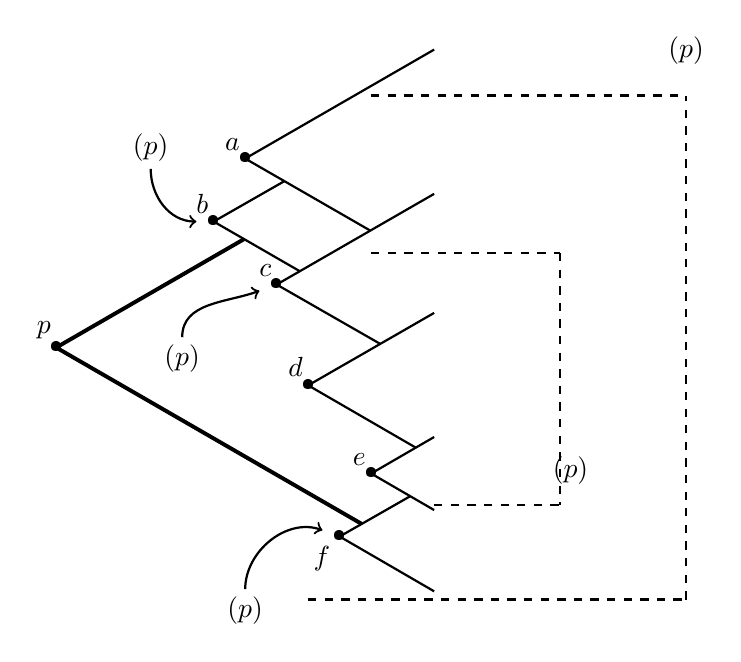
\begin{tikzpicture}[thick, scale=0.8]
        \node[label={[label distance = -3mm]160:$p$}]
        at (0.00, 0.00) {\textbullet};
        \node[label={[label distance = -3mm]160:$a$}]
        (a) at (3.00, 3.00) {\textbullet};
        \node[label={[label distance = -3mm]160:$b$}]
        (b) at (2.50, 2.00) {\textbullet};
        \node[label={[label distance = -3mm]160:$c$}]
        (c) at (3.50, 1.00) {\textbullet};
        \node[label={[label distance = -3mm]160:$d$}]
        at (4.00, -0.60) {\textbullet};
        \node[label={[label distance = -3mm]160:$e$}]
        at (5.00, -2.00) {\textbullet};
        \node[label={[label distance = -3mm]220:$f$}]
        (f) at (4.50, -3.00) {\textbullet};

        % e cone
        \draw (5.00, -2.00) -- (6.00, -2.58);
        \draw (5.00, -2.00) -- (6.00, -1.42);
        % f cone
        \draw (4.50, -3.00) -- (6.00, -3.87);
        \draw (4.50, -3.00) -- (5.62, -2.36);
        % d cone
        \draw (4.00, -0.60) -- (5.71, -1.59);
        \draw (4.00, -0.60) -- (6.00, 0.55);
        % c cone
        \draw (3.50, 1.00) -- (5.14, 0.06);
        \draw (3.50, 1.00) -- (6.00, 2.44);
        % a cone
        \draw (3.00, 3.00) -- (4.98, 1.86);
        \draw (3.00, 3.00) -- (6.00, 4.73);
        % b cone
        \draw (2.50, 2.00) -- (3.87, 1.21);
        \draw (2.50, 2.00) -- (3.62, 2.64);
        % p cone
        \draw[line width = 0.5mm] (0.00, 0.00) -- (4.85, -2.80);
        \draw[line width = 0.5mm] (0.00, 0.00) -- (2.98, 1.72);

        \draw[dashed] (6,-2.5) -- (8, -2.5)
        node[anchor=west, label=90:$\Cands(p)$] {};
        \draw[dashed] (8, 1.5) -- (8, -2.5);
        \draw[dashed] (5,1.5) -- (8, 1.5);

        \draw[dashed] (4, -4) -- (10, -4);
        \draw[dashed] (10, -4) -- (10, 4);
        \draw[dashed] (5, 4) -- (10, 4)
        node[anchor=south, label=$\Maxima(p)$] {};

        \node[label={[label distance = -3mm]270:$\low(p)$}]
        (low) at (3, -4) {};
        \draw[->] (low) edge[out=90,in=160] (f);

        \node[label={[label distance = -3mm]270:$\lcand(p)$}]
        (lc) at (2, 0) {};
        \draw[->] (lc) edge[out=90,in=200] (c);

        \node[label={[label distance = -3mm]90:$\up(p)$}]
        (up) at (1.5, 3) {};
        \draw[->] (up) edge[out=270,in=180] (b);
    \end{tikzpicture}
    \caption[Exemplo dos conjuntos utilizados no algoritmo]{Os pontos
        $c$, $d$ e $e$ pertencem a $\Cands(p)$, e todos os pontos exceto
        $p$ pertencem a $\Maxima(p)$. O ponto $b$ é $\up(p)$ e o ponto
        $f$ é $\low(p)$. O ponto $c$ é $\lcand(p)$.}
    \label{fig:parestatico:conjuntos}
\end{figure}